\documentclass[a4paper,12pt,fleqn]{article}
\usepackage[T1]{fontenc}
\usepackage{ucs}
\usepackage[utf8x]{inputenc}
\usepackage{ngerman}
\usepackage[ngerman]{babel}
\usepackage{lastpage}
\usepackage[pdftex]{color,graphicx}
\usepackage{listings}
\usepackage{pdflscape}
\usepackage{longtable}
\usepackage[inner=2cm,outer=2cm,top=1cm,bottom=1.5cm,includeheadfoot]{geometry}
\usepackage{fancyhdr}
\usepackage{url}
\usepackage{draftwatermark}
\usepackage{booktabs}
\usepackage{blindtext} 
\usepackage{framed} 
\usepackage{xcolor} 
\colorlet{shadecolor}{black} 
\usepackage{latexsym}

\usepackage{bbm}
\usepackage{enumitem}

\SetWatermarkText{Vertraulich}
\SetWatermarkScale{4}
\SetWatermarkLightness{0.9}

\usepackage{pgfgantt}
\usepackage{amsmath,amssymb,amsfonts,amstext}
\usepackage{floatflt}
\usepackage{tikz}
\usetikzlibrary[arrows,snakes,backgrounds,shapes]
\usetikzlibrary{through}
\usetikzlibrary{calc}
\usepackage{caption}
\usepackage{subcaption}

% highlighting
\usepackage{xcolor,soul}

%---- PageLayout
\pagestyle{fancy}

\setlength{\headsep}{10mm}

\usepackage{eso-pic}

%----------------------------------------------------------------------------
% HEADER --------------------------------------------------------------------
%----------------------------------------------------------------------------
\fancyhead[R]{
  
\includegraphics[width=100pt,keepaspectratio]{img/amedo2012.png}
}

\fancyhead[C]{ Wochenbericht KW 31 }

\fancyhead[L]{
  \begin{tabular}[b]{l}
  Christoph Gnip\\
  Projekt: PRPS-Evolution
  \end{tabular}
}

%Linie oben
\renewcommand{\headrulewidth}{0.5pt}
%----------------------------------------------------------------------------

%----------------------------------------------------------------------------
%----------------------------------------------------------------------------
%----------------------------------------------------------------------------
\fancyfoot[L]{Stand: \today}
\fancyfoot[C]{ EXTERN }
\fancyfoot[R]{\thepage{} von \pageref{LastPage}}

% Linie unten
\renewcommand{\footrulewidth}{0.5pt}
%----------------------------------------------------------------------------

% Import Macros  ------------------------------------------------------------
\newcommand\nn{\newline\newline}

%----------------------------------------------------------------------------
% Start the Document --------------------------------------------------------
%----------------------------------------------------------------------------
\begin{document}

\setlength{\headheight}{36pt}

\begin{titlepage}


%- the Title page --------------------------------------------------------
\begin{center}
%\vspace*{2.5cm}
{\Huge \textbf{Wochenbericht KW 31}\par}
\vspace{1cm}
{\Huge 29.7. - 4.8.2013\par}
\vspace{1cm}
{\Huge Projektwoche: 15\par}

\vspace{2cm}

\large{Erstellt durch}\\
\Large{\textbf{Christoph Gnip}}

\vspace{4cm}

\Large{\textbf{Extern}}

\vfill

{\normalsize Fachbereich Elektrotechnik und angewandte Naturwissenschaften\\
Westfälische Hochschule\\[2ex]Juni 2013}

\end{center}
\newpage

\end{titlepage}

%- Section 1 ----------------------------------------------------------------
\section[Allgemeines]{Allgemeines}
%
%Dieser Wochenbericht fasst die Projektwochen 12 und 13 zusammen. Die Ergebnisse dieses Zeitraums können so besser dargestellt werden.
%
%- Section 2 ----------------------------------------------------------------
\section[Fortschritt]{Projektfortschritt}
%
Bug in Shark 3.0b behoben. Er betraf die Ausgabe der Ergebnisse.
%Diese Woche wurde eine Tiefpassfilterung für den FPGA-entworfen und mittels Matlab/ Simulink getestet. Die Entwicklung an der Software wurde weitergeführt. So kann nun eine diskret~-~kontinuierliche Optimierung durchgeführt werden. Die Software wurde auf Shark 3.0b umgestellt.
%
%- Section 2.1 --------------------------------------------------------------
\subsection{Programmierung}
%
In dieser Woche wurden die vorgeschlagenen Modelle von Frau S. Winter implementiert. Sie sind als eigenständige Klassen eingeführt worden. Analog zu den in \cite{WinAmed13} beschriebenen Modellen wurde die Benennung der Klassen durchgeführt. Folgende Klassen wurden dem Namespace \textit{PRPSEvolution::Solve::Models} hinzugefügt:
\begin{enumerate}
\item SuWi_Modell_I
\item SuWi_Modell_II
\item SuWi_Modell_III
\end{enumerate}

%Es wurden mehrere Modellvariationen erstellt, die in der Optimierung eingesetzt werden. Es wurden Versuche mit unterschiedlichen Variablenvektoren angestellt, die dafür erstellten Modellvarianten können kontinuierliche sowie diskrete Variablen verarbeiten.
%
%- Section 2.2 --------------------------------------------------------------
%
\subsection{Visualisierung}
Mehrere neue Gnuplot-Skripte sind in dieser Woche entstanden.
%
%- Section 2.2 --------------------------------------------------------------
%
\subsection{Erkenntnisse aus der Visualisierung}
%
Keine guten Ergebnisse. Mehrere Lösungen laufen selten auf der gleich Ergebnis hinaus.
%
%- Section 2.3 --------------------------------------------------------------
\subsection{Auslegung der FIR-Filter}
%
%In Absprache mit M.~Hüther wurden in dieser Woche zwei Entwürfe für FIR-Filter gemacht. Diese werden im FPGA implementiert und realisieren eine Tiefpassfilterung der Daten. Der Entwurf wurde mittels Matlab erstellt, das verwendete Simulink Modell und sie Ergebnisse sind in Anhang~\ref{FirFilterResult} gezeigt. Die Implementation wurde nach einer ersten Abschätzung des Aufwands nach hinten verschoben. Es fehlen für die Synthese notwendige (mathematische) Libraries von Altera, die in der eingesetzten Version von Quartus nicht enthalten sind. Es gibt analog dazu verwendbare, freie Lösungen jedoch ist der Implementationsaufwand größer. Für die von M.~Hüther gefundene Lösung benötigt Ganzzahlige Koeffizienten, die bisher mit Matlab ermittelten müssen entsprechend transformiert werden.
%
%- Section 3 -----------------------------------------------------------------
\section{Probleme}
\label{Problems}
%
%Es kam bei der Umstellung auf die neue Shark Version 3.0 (beta) zu erheblichen Problemen. Die Bibliothek ließ sich zunächst nicht compilieren und der Vorgang brach mit mehreren hundert Fehlermeldungen ab. Die Fehler gingen von einer veralteten Version der Boost-Library zum Einen und der Verwendung der Verwendeten Compiler-Version (gcc 4.8) zum Anderen aus. Eine Deinstallation der veralteten Boost-Library und anschließender Rekompilierung der neuesten Version (Boost 1.54) mit dem gcc 4.8 hat das Problem behoben.
%
%- Appendix ------------------------------------------------------------------
%
%
%
\begin{appendix}

%----------------------------------------------------------------------------
%----------------------------------------------------------------------------
%----------------------------------------------------------------------------
\newpage

\begin{center}
	\huge{Anhänge}
\end{center}

\normalsize

%----------------------------------------------------------------------------
%----------------------------------------------------------------------------
%----------------------------------------------------------------------------
%\section{Filter Entwurf - Ergebnisse}
%\begin{landscape}
%\label{FirFilterResult}
%\begin{figure} [h]
         \centering
         \caption{ Ergebnisse des Filterentwurfs }
         \label{fig:1}
         \centering
         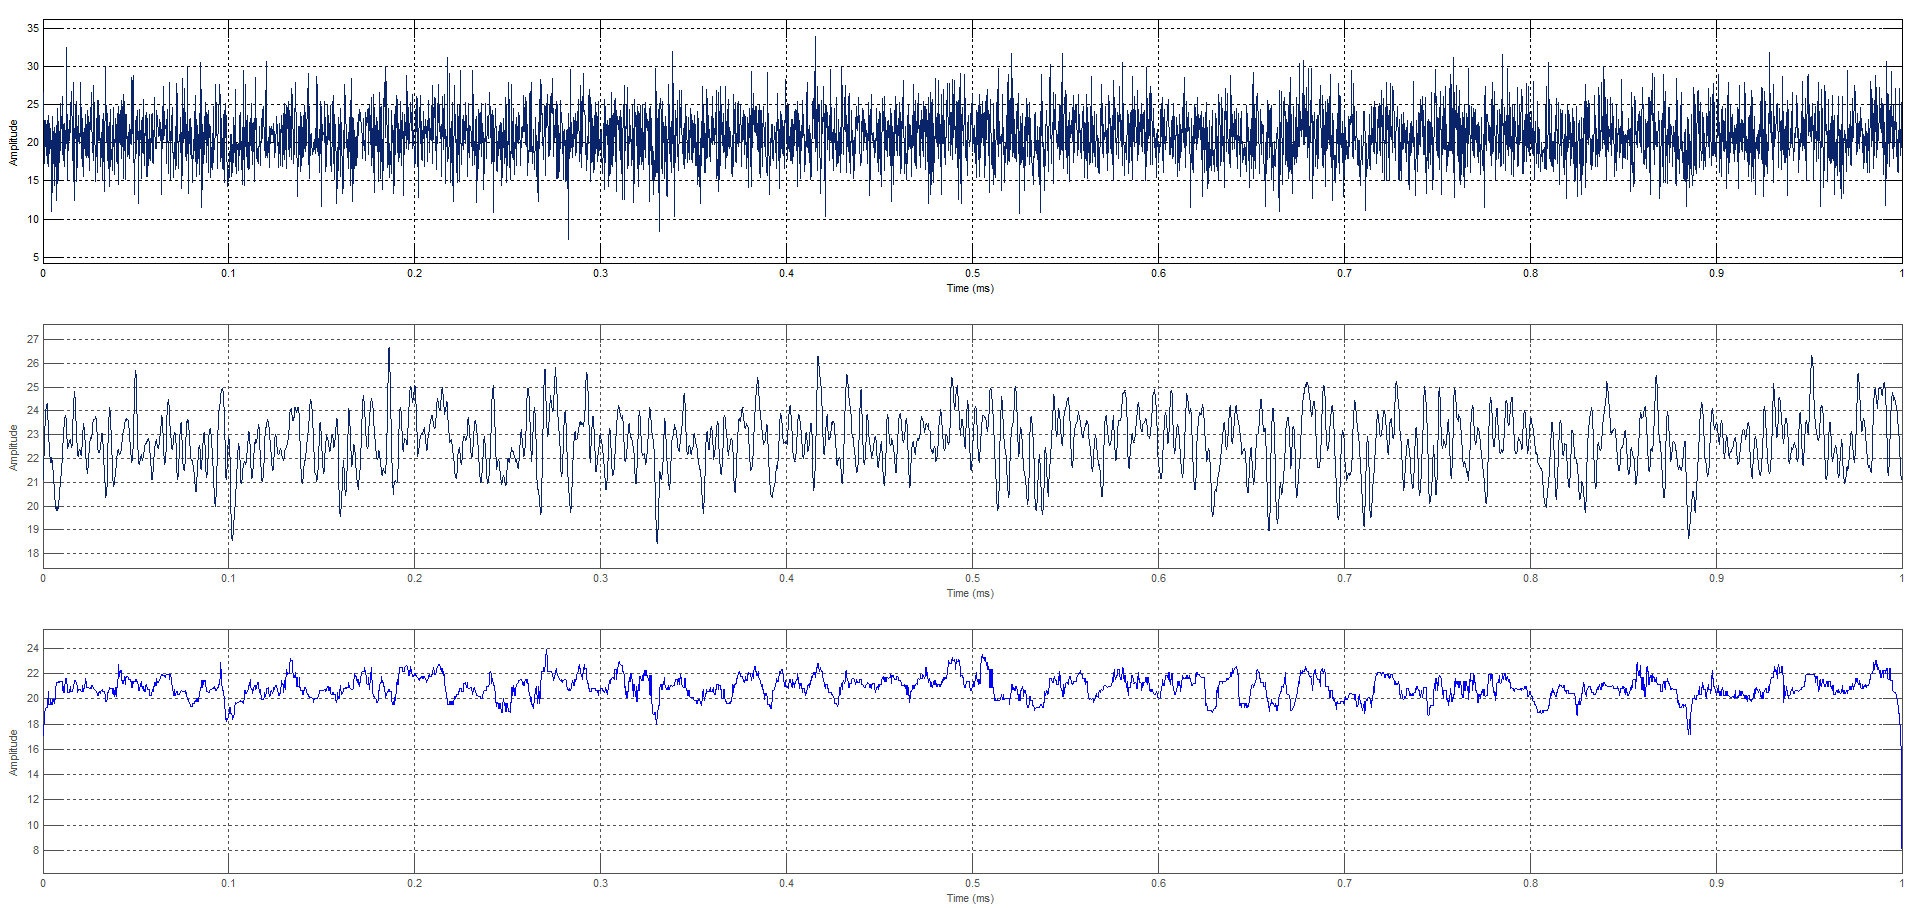
\includegraphics[width=.8\textwidth]{common/img/AmpGefiltert_small.png}\\
\vspace{0.5cm}
Die obere Kurve visualisiert die Rohdaten. Die mittlere Kurve ist das Ergebnis der Tiefpassfilterung für einen der vorgestellten Filter. Die untere Darstellung dient zum Vergleich mit der bisher eingesetzten Filterungsmethode (Median). Es wurden 4096 Messwerte für diese Analyse gesampelt.
\end{figure}
%---------------------------------------------------------------------------------------
\vspace{.5cm}
%---------------------------------------------------------------------------------------
\begin{figure} [h]
         \centering
         \caption{ Spektrum des Messsignals, vor und nach der Filterung  }
         \label{fig:2}
	     \centering
	     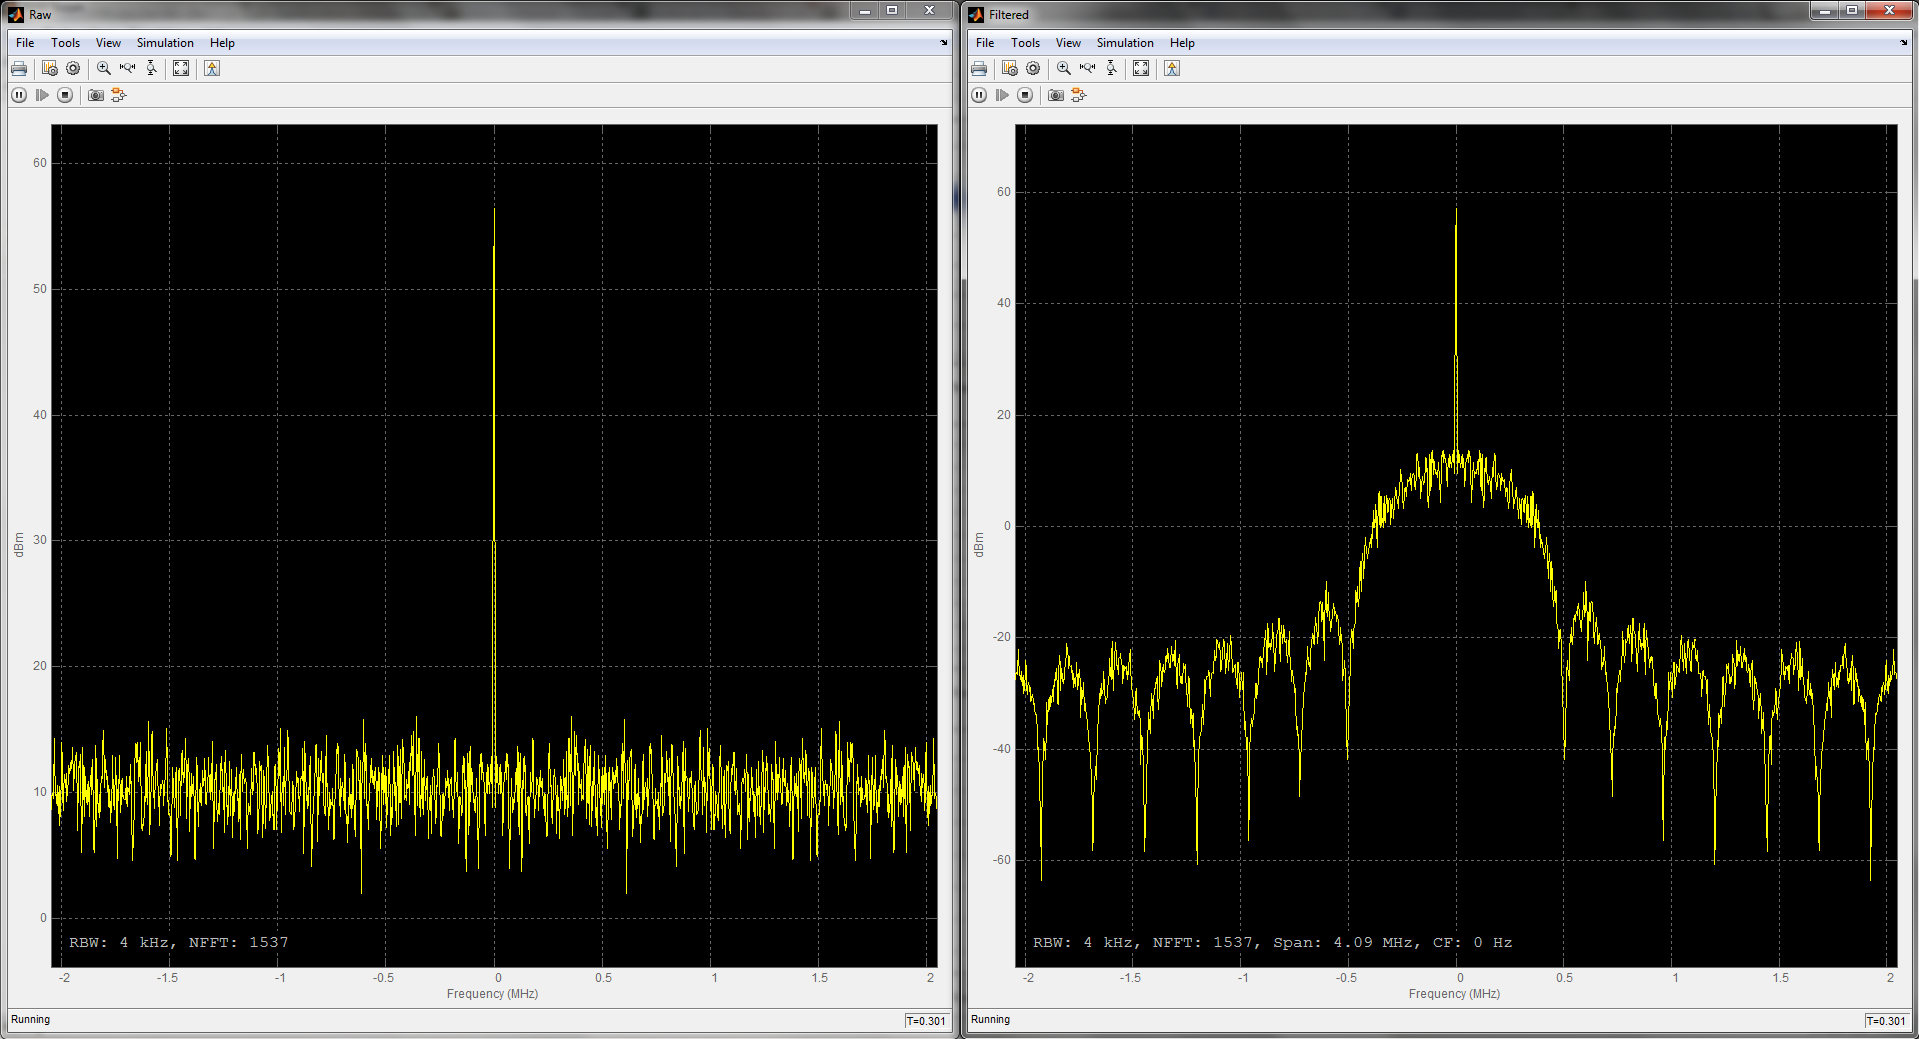
\includegraphics[width=.6\textwidth]{common/img/SpektrumAmp.PNG} \\
\vspace{.2cm}
Die Grafik zeigt das Spektrum des Messsignals der Amplitude. Im linken Bild ist das ungefilterte Signal und im Rechten das gefilterte.
%
\end{figure}
%---------------------------------------------------------------------------------------
\vspace{.5cm}
%---------------------------------------------------------------------------------------
\begin{figure} [h]
         \centering
         \caption{ Frequenzgänge der entworfenen Filter. Beide ähneln sich in den Parametern, verfügen jedoch über etwas unterschiedliche Eckfrequenzen. Als Entwurfsmethode wurde die sog. "Least-squares"-Methode verwendet. Diese Methode liefert gute Ergebnisse im Hinblick auf möglichst kleine Sidelobes und eine geringe Anzahl an Koeffizienten. }
         \label{fig:3}
%         
         \begin{subfigure}[t]{0.5\textwidth}
                 \centering
                 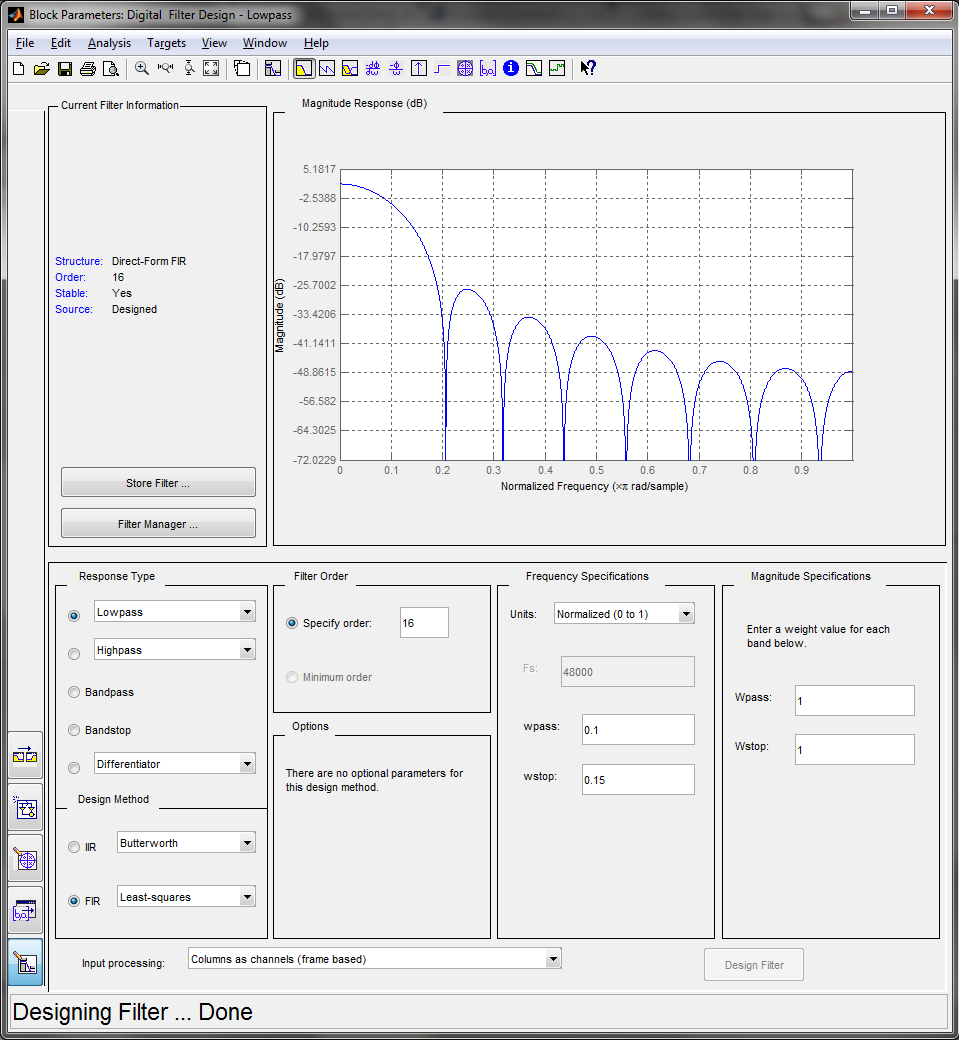
\includegraphics[width=\textwidth]{common/img/filter.png}
                 \vspace{.1cm}
                 \caption{Erstes Filter mit den Parametern wpass~=~0.1 und wstop~=~0.15. Das Ergebnis ist ein schmalbandigeres Filter. }
                 \label{fig:Filter1_A}\textit{}
         \end{subfigure}
%         
\qquad
         \begin{subfigure}[t]{0.5\textwidth}
                 \centering
                 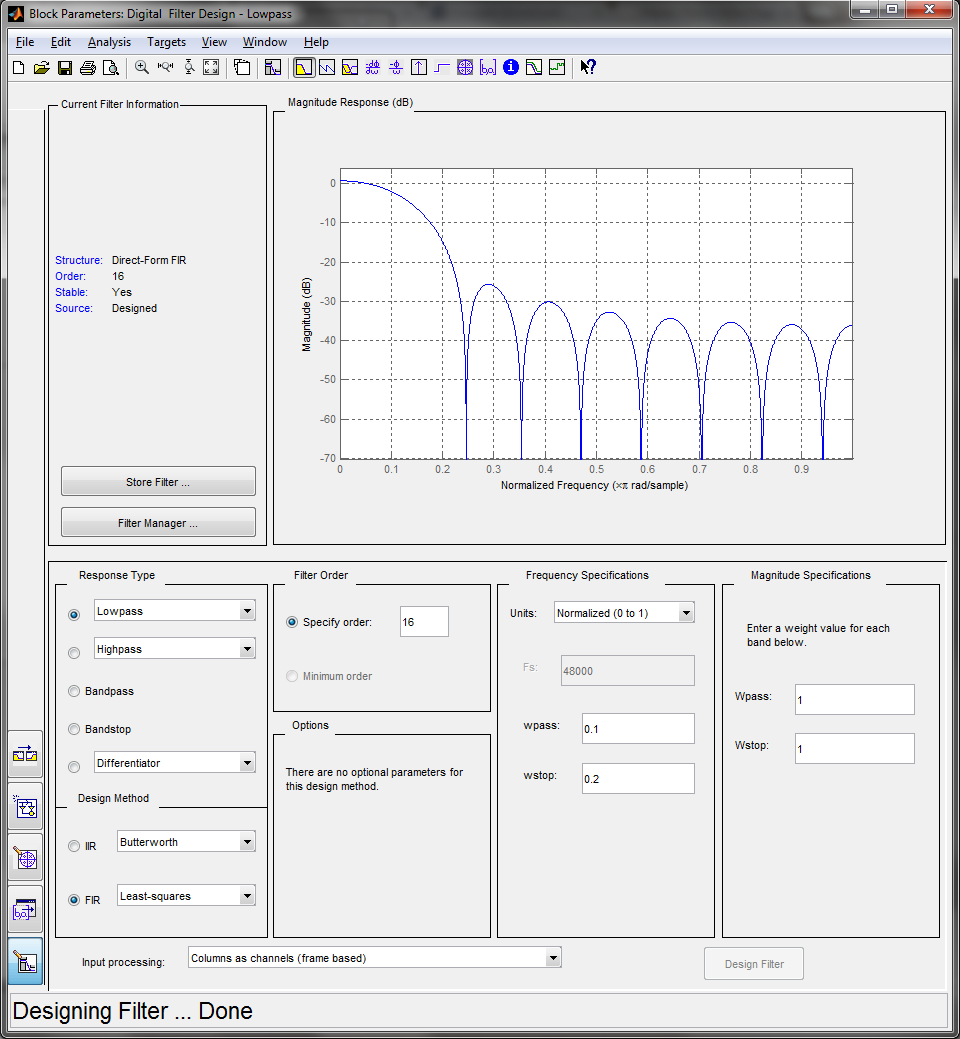
\includegraphics[width=\textwidth]{common/img/filter2.png}
                 \vspace{.1cm}
                 \caption{ Zweites Filter mit den Parametern wpass~=~0.1 und wstop~=~0.2. Der Durchlas bereich ist etwas breiter, dafür sind die Sidelobes stärker gedämpft }
                 \label{fig:Filter2_B}
         \end{subfigure}
%
\end{figure}
%---------------------------------------------------------------------------------------
%\end{landscape}

%----------------------------------------------------------------------------
%----------------------------------------------------------------------------
%----------------------------------------------------------------------------
\newpage
\begin{landscape}
	\section{Projektlaufplan KW 31}
	\label{sec:projectplan}
	\scalebox{.75}{
		\begin{ganttchart}[vgrid={draw=none,*1{gray, dashed}},
				hgrid=true,
				today=24,
				title height=1,
				y unit title=0.6cm,
				y unit chart=0.8cm,
				group right shift=0,
				group top shift=.3,
				group height=.3,
				milestone width=.8,
				group peaks={}{}{.2},
				incomplete/.style={fill=black!15}, %
				bar/.style={fill=white}, %
				today label={Heute},
				today rule/.style={dashed, thick}]{44}


\gantttitle{\textbf{2013}}{44} \\
\gantttitlelist{16,...,37}{2} \\
%-------------------------------------------------------------
\ganttgroup{Projekt Evaluation}{3}{14} \\
\ganttbar[progress=100, progress label font=\small\color{black!75},
	progress label anchor/.style={right=4pt}]{Installation der Umgebungen}{3}{6} \\
	
\ganttbar[progress=100, progress label font=\small\color{black!75},
	progress label anchor/.style={right=4pt},
	bar label font=\normalsize\color{black},
	name=rech]{Recherche}{3}{7} \\
	
\ganttmilestone[name=ms1]{Vorstellung der Ergebnisse}{7} \\
	
\ganttbar[progress=90, progress label font=\small\color{black!75},
	progress label anchor/.style={right=4pt},
	bar label font=\normalsize\color{black},
	name=pflichten]
	{Pflichtenheft}{5}{8} \\
	
\ganttmilestone[name=ms2]{Pflichtenheft fertig}{8} \\

\ganttbar[progress=100, progress label font=\small\color{black!75},
	progress label anchor/.style={right=4pt},
	bar label font=\normalsize\color{black},
	name=bNumVerf]
	{Einarbeitung num. Verfahren}{5}{16} \\

\ganttbar[progress=95, progress label font=\small\color{black!75},
	progress label anchor/.style={right=34pt},
	bar label font=\normalsize\color{black},
	name=bCMAES]
	{speziell CMA-ES}{7}{10} \\

\ganttmilestone[name=ms3]{Beurteilung num. Verfahren}{16} \\

\ganttlinkedbar[progress=100, progress label font=\small\color{black!75},
	progress label anchor/.style={right=34pt},
	bar label font=\normalsize\color{black}]
	{Shark Einarbeitung}{17}{18} \\

\ganttlinkedmilestone[name=ms7]{Abschluss Evaluation}{18} \\
	
%-------------------------------------------------------------
\ganttgroup{Erstellung Prototyp}{15}{26} \\
\ganttgroup{(optional)}{15}{18} \\
\ganttbar[progress=25, progress label font=\small\color{black!75},
	progress label anchor/.style={right=4pt},
	bar label font=\normalsize\color{black}]
	{(Entwurf digi. Filter)}{15}{15} \\

\ganttlinkedbar[progress=10, progress label font=\small\color{black!75},
	progress label anchor/.style={right=4pt},
	bar label font=\normalsize\color{black},
	name=bImpFPGA]
	{(Implementation FPGA)}{16}{18} \\

\ganttmilestone[name=ms4]{(Verifikation dig. Filter)}{18} \\
	
\ganttbar[progress=90, progress label font=\small\color{black!75},
	progress label anchor/.style={right=4pt},
	bar label font=\normalsize\color{black},
	name=bImplAlgo]
	{Implementation Algorithmus}{15}{26} \\

\ganttlinkedmilestone[name=ms5]{Implementation Done}{26} \\

%-------------------------------------------------------------
\ganttgroup{Verifikation}{27}{34} \\
\ganttbar[progress=10, progress label font=\small\color{black!75},
	progress label anchor/.style={right=4pt},
	bar label font=\normalsize\color{black},
	name=bVerf]
	{Durchf\"uhrung Verifikation}{27}{34} \\

\ganttlinkedmilestone[name=ms6]{Verifikation Done}{34} \\

%-------------------------------------------------------------
\ganttgroup{Projektdokumentation}{35}{42} \\

\ganttbar[progress=0, progress label font=\small\color{black!75},
	progress label anchor/.style={right=4pt},
	bar label font=\normalsize\color{black},
	name=thesis]
	{Thesis schreiben}{35}{42} \\
	
\ganttmilestone[name=msthesis,milestone label font=\color{red}, 
	milestone/.style={fill=red}]{Abgabe}{42}

%\ganttlink{ms7}{bImplAlgo}
\ganttlink{bImpFPGA}{ms4}
\ganttlink{bNumVerf}{ms3}
\ganttlink{bCMAES}{ms3}
\ganttlink{rech}{ms1}
\ganttlink{pflichten}{ms2}
\ganttlink{thesis}{msthesis}

	\end{ganttchart}
		}
\end{landscape}

%----------------------------------------------------------------------------

\end{appendix}


\newpage
%- Bibliography --------------------------------------------------------------
\bibliographystyle{ieeetr}
\bibliography{../bib/mathesis_collection1}

\end{document}